\begin{boiboiboite}
	\propeau
	\propair
\end{boiboiboite}

\subsubsection{Cycle de Rankine surchauffé}
\label{exo_porcheville_rankine}

\begin{comment}
	Quelques données pour cette centrale trouvées sur le web :
		1.800 tonnes/heure
		Fioul 10×plus cher que le charbon (1000 euros/tonne vs 100 euros)
		Chaque chaudière, 545° 180 bar, 130t fioul/heure
		Pression entrante turbines 150 bars
		Température de l’eau vers la seine: 3°C
		Charbon environ 35 MJ/kg
\end{comment}

	La centrale EDF de Porcheville (\cref{fig_porcheville}) reçoit de la chaleur issue de la combustion de fioul, et utilise un cycle à vapeur pour alimenter une génératrice électrique.
	
	\begin{figure}
		\begin{center}
			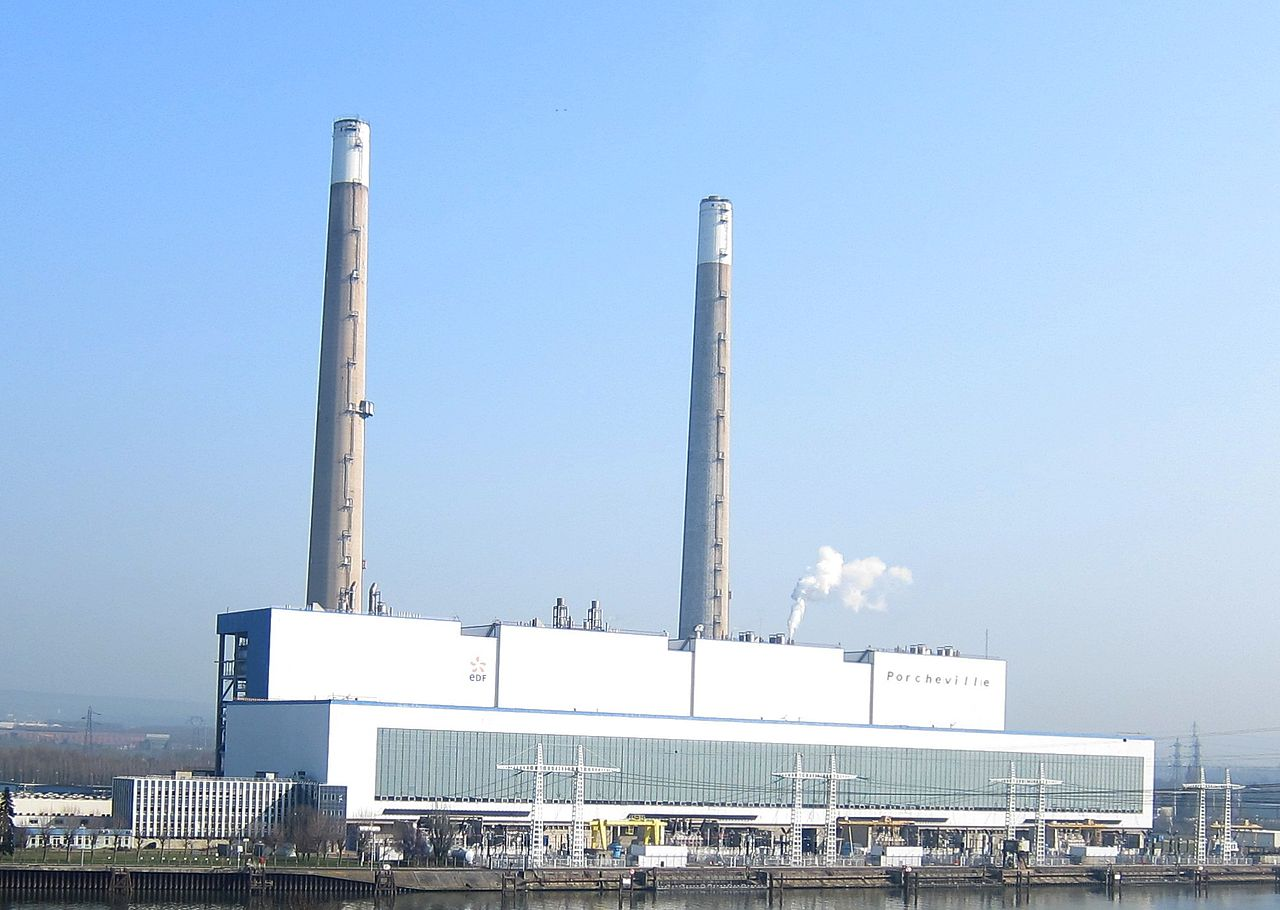
\includegraphics[width=8cm]{images/porcheville.jpg}
			\vspace{-0.5cm}%handmade
		\end{center}
		\supercaption{Centrale électrique de Porcheville, alimentée au charbon jusqu’en 1987 et fonctionnant désormais au fioul. Elle sert principalement les demandes de pointe.}{Photo \cczero \oc}
		\label{fig_porcheville}
	\end{figure}
	
	Dans la centrale l’eau évolue entre les pressions de~\SI{0,1}{\bar} et~\SI{140}{\bar}. La vapeur atteint~\SI{545}{\degreeCelsius}, et les turbines ont une efficacité isentropique de~\SI{80}{\percent}.

	Pour les besoins de l’exercice, nous considérons que le cycle est basé sur un cycle de Rankine surchauffé.
	
	\begin{enumerate}
		\item Schématisez le circuit physique de l’eau dans la centrale ; tracez le cycle suivi sur un diagramme température-entropie, de façon qualitative (c’est à dire sans représenter les valeurs numériques) en y représentant aussi la courbe de saturation.
		\item Quelle est l’enthalpie de l’eau à la sortie des turbines ?
		\item Quelle est l’enthalpie de l’eau à la sortie des pompes ?
		\item	Quel est le rendement thermodynamique de l’installation ?
		\item Quelle est la consommation spécifique de l’installation, c’est-à-dire la masse de vapeur ayant traversé la turbine lorsque l’installation a généré \SI{1}{\kWh} d’énergie mécanique ?
		\item Quel débit horaire de vapeur faut-il faire circuler dans le circuit pour obtenir une puissance mécanique de~\SI{60}{\mega\watt} ?
	\end{enumerate}


\subsubsection{Mise en place d’une resurchauffe}
\label{exo_porcheville_resurchauffe}

	L’installation de Porcheville décrite dans l’exercice~\ref{exo_porcheville_rankine} est modifiée pour accueillir une série de tubes de resurchauffe. La détente de l’eau est interrompue à~\SI{18}{\bar} dans la turbine, et la vapeur est ramenée à la température maximale du cycle (c’est-à-dire \SI{545}{\degreeCelsius}).
	
	La centrale est alimentée au fioul lourd dit «~TBTS~», de masse volumique \SI{1050}{\kilogram\per\metre\cubed} et de pouvoir calorifique \SI{40,2}{\mega\joule\per\kilogram}.
	
	L’air utilisé pour la combustion pénètre dans la chaudière à température de~\SI{15}{\degreeCelsius} et pression de~\SI{1}{\bar}. Il est porté à température de~\SI{820}{\degreeCelsius} par combustion à pression constante, avant de passer autour des conduits d’eau. Lorsqu’il quitte la chaudière, sa température est de~\SI{180}{\degreeCelsius}.
	
	\begin{enumerate}
		\item Quel est le nouveau rendement thermique de la centrale ?
		\item Quelle est sa nouvelle consommation spécifique ?
		\item Quel débit d’air faut-il admettre dans la chaudière pour maintenir une puissance mécanique nette de \SI{60}{\mega\watt} ?
		\item Quelle est l’efficacité de la chaudière ?
		\item Quel est le débit volumique horaire de carburant ?
		\item Un/e ingénieur/e propose de faire passer le conduit d’air d’admission au travers des gaz d’échappement (sans pourtant les mélanger) pour augmenter la température de l’air avant combustion. Cela vous paraît-il être une bonne idée ?
	\end{enumerate}
	

\subsubsection{Cycle avec régénération}
\label{exo_brise_glace}

	Dans un navire brise-glace polaire (\cref{fig_50letpodeby}), une installation à vapeur alimente les hélices à partir d’un réacteur nucléaire.

	\begin{figure}
		\begin{center}
			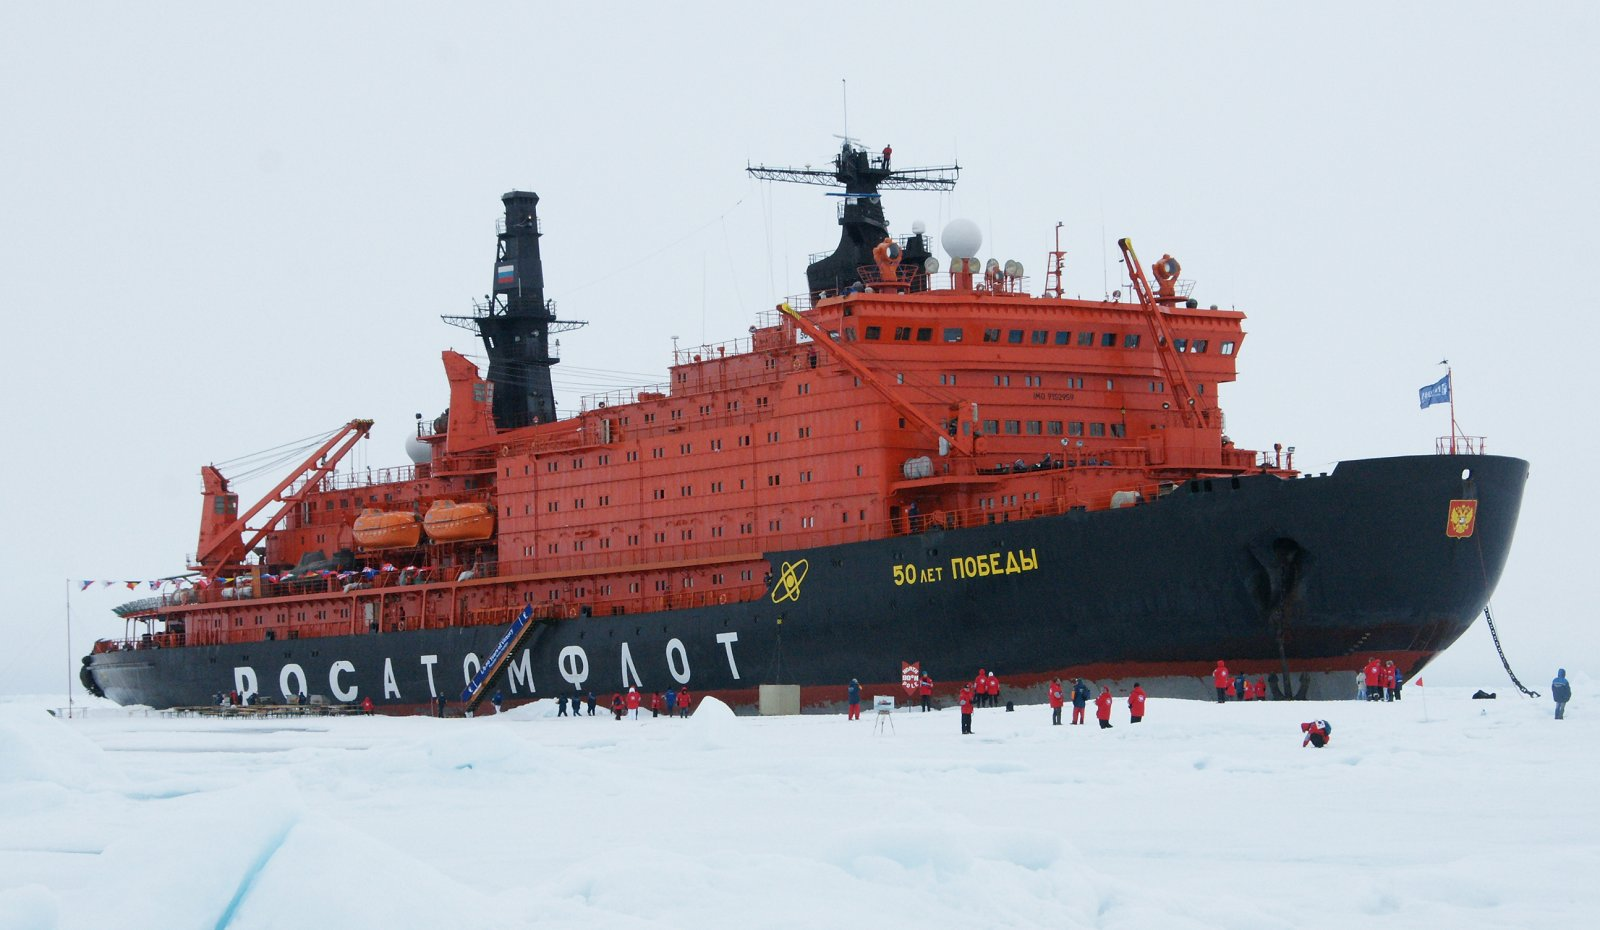
\includegraphics[width=11cm]{images/50letpodeby.jpg}
		\end{center}
		\supercaption{Le 50 Let Podeby, brise-glace de~\SI{25 000}{\tonne} à propulsion nucléo-turbo-électrique (deux réacteurs de~$\SI{171}{\mega\watt}_{\text{chaleur}}$, trois moteurs de~$\SI{17,6}{\mega\watt}_{\text{méch.}}$). Sa construction a débuté en 1989 mais il n’est entré en service qu’en 2007.}{\wcfile{50letPob_pole.JPG}{Photo} \ccbysa par \wcu{Kiselev d}}
		\label{fig_50letpodeby}
	\end{figure}

	Le cycle est basé sur un cycle de Rankine surchauffé à~\SI{310}{\degreeCelsius} (par contact avec les conduites avec l’eau pressurisée qui, elle, traverse le réacteur), entre les pressions de~\num{30} et~\SI{0,5}{\bar}\footnote{En réalité, entre \num{29} et~\SI{0,75}{\bar}, valeurs qui ne sont pas tabulées dans nos abaques.}. 
	
	Pour ne pas surcharger cet exercice, nous considérons que la turbine est parfaitement isolée et isentropique.

	\begin{enumerate}
		\item Quel est le rendement thermodynamique de l’installation ?
		\item On définit la consommation spécifique de vapeur comme l’inverse de la puissance nette de l’installation. C’est la masse de vapeur ayant traversé la turbine lorsque l’installation a généré \SI{1}{\kWh} d’énergie mécanique.\\
			Quelle est la consommation spécifique de l’installation ?
	\end{enumerate}

	Un/e ingénieur/e propose de modifier le cycle pour le rendre régénératif, en prélevant de la vapeur de la turbine pour l’insérer dans le circuit de compression.
	
	Il/elle propose de séparer la compression en deux étapes, l’une de~\num{0,5} à~\SI{6}{\bar}, et la seconde de~\num{6} à~\SI{30}{\bar} ; et d’insérer la vapeur prélevée entre les deux pompes. Le débit de vapeur prélevé est tel que l’eau à la sortie du mélangeur est exactement à saturation.
	
	Pour simplifier nos calculs, nous considérons que la puissance de pompage n’est pas modifiée par la régénération (une approximation sans grande incidence).
	
	\begin{enumerate}	
		\shift{2}
		\item Schématisez l’installation proposée (c’est-à-dire le circuit physique suivi par la vapeur).
		\item Représentez le cycle thermodynamique sur un diagramme température-entropie de façon qualitiative en y représentant aussi la courbe de saturation de l’eau.
		\item Quelle proportion du débit de vapeur faudrait-il prélever à~\SI{6}{\bar} dans la turbine, pour chauffer l’eau à saturation entre les deux pompes ?
		\item La puissance aux hélices augmente-t-elle ou diminue-t-elle, et de combien ?
		\item Le rendement de l’installation augmente-t-il ou diminue-t-il, et de combien ?
	\end{enumerate}

\exercisesolutionpage
\titreresultats
	
	\begin{description}
		\item [\ref{exo_porcheville_rankine}] 
						\tab 1) Voir les figures~\ref{fig_cycle_rankine_surchauffe} et~\ref{fig_ts_lv_rankine_surchauffe} ;
						\tab 2) Avec $s_\E = s_\D = \SI{6,5399}{\kilo\joule\per\kilogram}$ et $\eta_\text{T} = \SI{80}{\percent}$, nous obtenons $h_\E = \SI{2287,7}{\kilo\joule\per\kilogram} $ comme à l’exemple~\ref{exemple_turbine_centrale} ;
						\tab 3) Avec l’\cref{eq_pompe_liquide} nous obtenons $h_\B = \SI{205,9}{\kilo\joule\per\kilogram}$ comme à l’exemple~\ref{exemple_pompe_centrale} ;
						\tab 4) $\eta_\text{thermique} = \left|\frac{(h_\E - h_\D) + (h_\B - h_\A)}{(h_\D - h_\B)}\right| = \SI{35,29}{\percent}$ (\ref{def_rendement_moteur}) ;
						\tab 5) $SSC = \SI[per-mode = symbol]{3,15}{\kilogram\per\kilo\watt\per\hour}$ ;
						\tab 6) $\dot{m}_\text{eau} = \SI{52,5}{\kilogram\per\second}$.
		\item [\ref{exo_porcheville_resurchauffe}] 
						\tab 1) $h_{\D2} = \SI{2960,8}{\kilo\joule\per\kilogram}$, $h_{\E2} = \SI{3570,3}{\kilo\joule\per\kilogram}$, $h_\F = \SI{2642,7}{\kilo\joule\per\kilogram}$, ainsi l’efficacité atteint $\eta_\text{thermique 2} = \SI{36,31}{\percent}$ (\SI{+1}{pt}, une amélioration déjà appréciable) ;
						\tab 2) $SSC_2 = \SI[per-mode = symbol]{2,576}{\kilogram\per\kilo\watt\per\hour}$ (\SI{-18}{\percent}, un beau résultat) ;
						\tab 3) Dans la chaudière, la chaleur perdue par l’air est gagnée par l’eau : $\dot m_\text{air} = \frac{-\dot Q_\text{eau}}{c_p \ \Delta T} = \frac{\dot W_\net}{\eta_\text{thermique}} \frac{1}{c_p \ (T_\text{air 3} - T_\text{air 2})}	 = \SI{256,9}{\kilogram\per\second}$.
						\tab 4) $\eta_\text{chaudière} = \frac{\dot Q_\text{eau}}{\dot Q_\text{reçue par l’air}} = \SI{79,5}{\percent}$ 
						\tab 5) $\dot{V}_\text{carb.} = \frac{\dot Q_\text{reçue par l’air}}{\rho_\text{carburant} c_\text{carburant} \eta_\text{chaudière}} = \SI{17,7}{\metre\cubed\per\hour}$.
						\tab 6) C’est une excellente idée. On réduit ainsi la chaleur emportée par les gaz d’échappement à la sortie de la chaudière, ce qui a pour effet immédiat d’augmenter $\eta_\text{chaudière}$.
						
		\item [\ref{exo_brise_glace}]
						\tab 1) Avec le schéma des figures figures~\ref{fig_cycle_rankine_surchauffe} et~\ref{fig_ts_lv_rankine_surchauffe}, $h_\A = \SI{340,5}{\kilo\joule\per\kilogram}$, $h_\B = \SI{343,54}{\kilo\joule\per\kilogram}$, $h_\D = \SI{3017,4}{\kilo\joule\per\kilogram}$, $h_\E = \SI{2284,5}{\kilo\joule\per\kilogram}$, ainsi $\eta_\text{thermique} = \SI{27,294}{\percent}$ ;
						\tab 2) $SSC = \SI[per-mode = symbol]{4,93}{\kilogram\per\kilo\watt\per\hour}$ ;
						\tab 3) Voir \cref{fig_cycle_prélèvement_vapeur} ;
						\tab 4) Voir \cref{fig_ts_lv_prelevement_vapeur} ;
						\tab 5) $h_\text{prélèvement} = \SI{2673,9}{\kilo\joule\per\kilogram}$, $h_\text{pré-mélange} = \SI{341,1}{\kilo\joule\per\kilogram}$, $h_\text{post-mélange} = \SI{670,4}{\kilo\joule\per\kilogram}$ : Ainsi la proportion permettant de saturer l’eau après mélange est $z = \SI{14,1}{\percent}$ ;
						\tab 6) $w_\text{net~2} = \SI{-674,87}{\kilo\joule\per\kilogram}$ (\SI{-9,2}{\percent} : drame !) ;
						\tab 7) $q_\text{chaud.} = \SI{2344,4}{\kilo\joule\per\kilogram}$, ainsi $\eta_\text{inst.~2} = \SI{28,786}{\percent}$ (\SI{+1,49}{pt} : est-ce vraiment désirable dans cette application ?).
	\end{description}
